\section{Spin-Boson Model as the First Worked Example}
\label{sec:spin_boson_example}

\paragraph{Role of this section.}
The general duality framework is model-independent.
The spin-boson qubit is introduced here as the first concrete realization because it is both
physically canonical and analytically closed
\cite{leggettDynamicsDissipativeTwostate1987,cresserWeakUltrastrongCoupling2021a}.
The objective is not to claim universality from one model, but to show how the representative maps
become operational with explicit formulas.

\subsection{From Hamiltonian to closed mean-force coordinates}

We take
\begin{align}
  H_Q &= \frac{\omega_q}{2}\sigma_z, \\
  H_X &= \sum_k \omega_k b_k^\dagger b_k, \\
  f(\theta) &= \cos\theta\,\sigma_z - \sin\theta\,\sigma_x, \\
  B &= \sum_k c_k(b_k+b_k^\dagger), \\
  H_{\mathrm{int}} &= g\,f(\theta)\otimes B,
\end{align}
so \(H_{\mathrm{tot}}=H_Q+H_X+H_{\mathrm{int}}\).
Using Definition~\ref{def:influence_operator},
\begin{equation}
  \frac{\bar{\rho}_Q(\beta)}{Z_X(\beta)}
  = e^{-\beta H_Q/2}\,e^{S_\beta}\,e^{-\beta H_Q/2}.
\end{equation}
For Gaussian baths, closure compresses bath dependence into two real response scalars,
\(\Sigma_z(\beta,g)\) and \(\Sigma_\perp(\beta,g)\)
\cite{cresserWeakUltrastrongCoupling2021a,cerisolaQuantumClassicalCorrespondence2024,mccaulMeanForceHamiltoniansInfluence2026}.
Define \(c=\cos\theta\), \(s=\sin\theta\), and
\begin{align}
  \chi &:= s\sqrt{c^2\Sigma_\perp^2+s^2\Sigma_z^2}, \\
  \gamma(\chi) &:= \frac{\tanh\chi}{\chi}, \\
  \Theta &:= \operatorname{arctanh}\!\big(\gamma(\chi)s^2\Sigma_z\big)-\frac{\beta\omega_q}{2}, \\
  m_z &:= \tanh\Theta, \qquad r:=|\tanh\chi|, \\
  \tan\eta &:= -\cot\theta\,\frac{\Sigma_\perp}{\Sigma_z}.
\end{align}
This split has immediate physical meaning:
\(\chi\) controls radius/purity (how mixed the reduced state is), while \((\Theta,\eta)\) control
orientation (where the Bloch vector points).

With one-channel scaling \(K(u)=g^2K_0(u)\),
\begin{equation}
  \Sigma_z=g^2\Sigma_z^{(0)},\qquad
  \Sigma_\perp=g^2\Sigma_\perp^{(0)},
\end{equation}
so
\begin{align}
  \chi(\beta,g,\theta) &= g^2\chi_0(\beta,\theta), \\
  g_\star(\beta,\theta) &= \chi_0^{-1/2}, \\
  g^\vee &= \frac{g_\star^2}{g}.
\end{align}

\subsection{Why the strong-coupling limit is analytically easy}

Write the influence generator as
\begin{equation}
  S = \Delta_0\I + \Delta_z \sigma_z + \Delta_\perp
  (\sigma_x\cos\phi_f + \sigma_y\sin\phi_f),
\end{equation}
and let \(M=S-\Delta_0\I\), so \(M^2=\chi^2\I\).
Then exactly
\begin{equation}
  e^S=e^{\Delta_0}\cosh\chi\,\big(\I+\gamma M\big),
  \qquad
  \gamma=\frac{\tanh\chi}{\chi}.
\end{equation}
This closed form is the main practical simplification: in the strong sector \(\chi\gg1\),
one reads off asymptotics directly from elementary functions without extra resummation.
The radial saturation \(r\to1\) follows immediately from \(\tanh\chi\to1\).

\subsection{Dual transfer to low-temperature control}

At fixed \(g\), low-temperature analysis can be difficult because \(\chi_0(\beta,\theta)\)
develops strong structure as \(\beta\to\infty\).
If \(\chi_0\to\infty\), then
\begin{equation}
  g^\vee=\frac{1}{\chi_0 g}\to0,
  \qquad
  \chi(\beta,g^\vee,\theta)=\chi(\beta,g,\theta)^{-1}\to0.
\end{equation}
So the hard strong-\(\chi\) sector at \((\beta,g)\) is evaluated through the weak-\(\chi\)
expansion of the dual representative \((\beta,g^\vee)\).
This is the central control payoff of the dual map.

\subsection{Canonical threshold and angle-resolved phase structure}
\label{subsec:ground_state_phase_transitions_v2}

To obtain closure-exact critical couplings, first specialize to the canonical channel
\(\theta=\pi/2\) (so \(c=0\), \(s=1\)).
Then
\begin{equation}
  \chi(\beta,g)=g^2\Sigma_z^{(0)}(\beta;s),
  \qquad
  \Theta(\beta,g)=\chi(\beta,g)-\frac{\beta\omega_q}{2},
\end{equation}
which gives
\begin{equation}
  m_z(\beta,g;s)=\tanh\!\left[g^2\Sigma_z^{(0)}(\beta;s)-\frac{\beta\omega_q}{2}\right].
\end{equation}
Define
\begin{equation}
  \lambda_s:=\lim_{\beta\to\infty}\frac{\Sigma_z^{(0)}(\beta;s)}{\beta}.
\end{equation}
When \(\lambda_s\in(0,\infty)\), the \(T=0\) order parameter is
\begin{equation}
  m_0(g;s)=\operatorname{sgn}\!\left(g^2\lambda_s-\frac{\omega_q}{2}\right),
\end{equation}
with exact critical coupling
\begin{equation}
  g_c^2(s)=\frac{\omega_q}{2\lambda_s}.
  \label{eq:gc_exact_lambda_v2}
\end{equation}
For
\begin{equation}
  J_s(\omega)=2g^2\,\omega_c^{1-s}\omega^s e^{-\omega/\omega_c},\qquad s>0,
\end{equation}
one gets
\begin{equation}
  \lambda_s=2\omega_c\Gamma(s),
  \qquad
  g_c^2(s)=\frac{\omega_q}{4\omega_c\Gamma(s)}.
  \label{eq:gc_exact_gamma_v2}
\end{equation}
This spectral dependence is exact for the canonical \(\theta=\pi/2\) slice of the closure model.

\paragraph{Angle dependence from the same closed equations.}
For generic \(\theta\), define
\begin{equation}
  D_0(\beta,\theta):=s^2\Sigma_z^{(0)}(\beta,\theta),\qquad
  X_0(\beta,\theta):=\chi_0(\beta,\theta),
\end{equation}
and
\begin{equation}
  Q_\theta(\beta):=\frac{D_0(\beta,\theta)}{X_0(\beta,\theta)}\in(0,1].
\end{equation}
The sign-change condition \(m_z=0\) (\(\Theta=0\)) becomes
\begin{equation}
  Q_\theta(\beta)\,\tanh(g_c^2X_0)=\tanh\!\left(\frac{\beta\omega_q}{2}\right),
  \label{eq:gc_angle_condition_v2}
\end{equation}
so
\begin{equation}
  g_c^2(\beta,\theta)=\frac{1}{X_0}\operatorname{arctanh}
  \!\left[\frac{\tanh(\beta\omega_q/2)}{Q_\theta(\beta)}\right],
  \label{eq:gc_angle_finite_beta_v2}
\end{equation}
only if \(\tanh(\beta\omega_q/2)<Q_\theta(\beta)\); otherwise there is no finite \(g_c\).
As \(\beta\to\infty\), a finite threshold requires \(Q_\theta\to1\), i.e. the transverse sector must
vanish. In practice, the finite-threshold region contracts toward the canonical axis.

\begin{figure}[tbp]
  \centering
  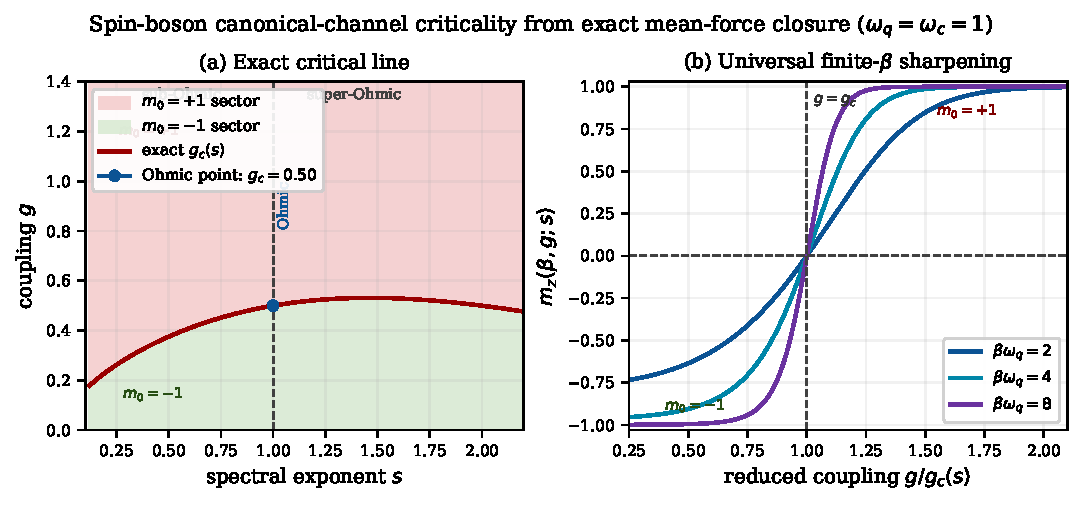
\includegraphics[width=\columnwidth]{../figures/hmf_spin_boson_phase_diagram.pdf}
  \caption{
  Spin-boson closure criticality on the canonical channel.
  \textbf{(a)} Exact spectral-class critical line
  \(g_c(s)=\sqrt{\omega_q/(4\omega_c\Gamma(s))}\).
  \textbf{(b)} Universal finite-\(\beta\) sharpening in reduced coupling
  \(x=g/g_c(s)\), with transition pinned at \(x=1\).
  }
  \label{fig:spin_boson_phase_diagram_v2}
\end{figure}

\begin{figure}[tbp]
  \centering
  
\includegraphics[width=\columnwidth]{../figures/hmf_spin_boson_angle_phase_map.pdf}
  \caption{
  Ohmic (\(s=1\)) angle dependence of the closure threshold.
  \textbf{(a)} Existence ratio \(Q_\theta(\beta)\) compared with
  \(\tanh(\beta\omega_q/2)\) (dashed).
  \textbf{(b)} Finite-\(\beta\) \(g_c(\beta,\theta)\) from
  Eq.~\eqref{eq:gc_angle_finite_beta_v2}; points with no finite solution are omitted.
  The threshold corridor narrows toward \(\theta=\pi/2\) as temperature is lowered.
  }
  \label{fig:spin_boson_angle_phase_map_v2}
\end{figure}

\paragraph{Interpretive note.}
The phase line \(g_c(s)\) is a zero-temperature closure boundary.
It is distinct from the finite-temperature crossover line \(g_\star(\beta,\theta)\) from \(\chi=1\).
The former separates asymptotic sectors of the canonical channel; the latter controls branch exchange
within finite-\(\beta\) calculations.

\paragraph{Scope relative to full spin-boson criticality.}
These \(g_c\) expressions are closure-level representative thresholds.
They are not a replacement for full spin-boson universality results. For the unbiased model, the
established phenomenology includes Ohmic KT criticality and no localization transition in the
super-Ohmic case \cite{leggettDynamicsDissipativeTwostate1987,weissQuantumDissipativeSystems2012}.
For sub-Ohmic dissipation, nonperturbative NRG/QMC and analytic studies report a genuine transition
with \(s\)-dependent critical behavior \cite{bullaQuantumPhaseTransitionSubohmic2003,vojtaQuantumPhaseTransitionsSubohmic2005,winterQuantumPhaseTransitionSubohmic2009,chinGeneralizedPolaronAnsatz2011,bullaNumericalRenormalizationGroup2008}.
The present angle-resolved map is therefore a duality-geometry statement inside the mean-force
closure, to be benchmarked against those full-model results rather than identified with them.

\subsection{Entropy geometry and dual representative map}

For any qubit state of Bloch radius \(r\),
\(\lambda_\pm=(1\pm r)/2\), so
\begin{equation}
  S_Q=-\sum_{\pm}\lambda_\pm\log\lambda_\pm.
\end{equation}
Using \(r=|\tanh\chi|\),
\begin{equation}
  S_Q(\beta,g,\theta)
  =h_2\!\left(\frac{1+|\tanh\chi(\beta,g,\theta)|}{2}\right),
\end{equation}
where \(h_2\) is the binary entropy.
Under \(g\mapsto g^\vee\), \(\chi\mapsto\chi^{-1}\), hence
\begin{equation}
  S_Q(\beta,g^\vee,\theta)
  =h_2\!\left(\frac{1+|\tanh(\chi^{-1})|}{2}\right).
\end{equation}
This is an exact analytic map between partner representatives.

Asymptotically,
\begin{equation}
  S_Q(\chi)=\log2-\frac{\chi^2}{2}+O(\chi^4),\quad \chi\to0,
\end{equation}
\begin{equation}
  S_Q(\chi)=\bigl(1+2\chi\bigr)e^{-2\chi}+O(e^{-4\chi}),\quad \chi\to\infty.
\end{equation}
So strong-branch entropy can be evaluated as a weak-branch expansion in \(\chi^\vee=\chi^{-1}\).

\paragraph{Connection to earlier spin-boson literature.}
The trends above are consistent with analytical and numerical studies of spin-boson entanglement and
localization diagnostics
\cite{costiEntanglementQubitEnvironment2003,koppUniversalMeasurableEntanglement2007,lehurEntanglementEntropyDecoherence2008,beraStabilizingSpinCoherence2014,beraGeneralizedMultipolaron2014}.
The distinct contribution here is the closed representative map that links the two branches by
\(\chi^\vee=\chi^{-1}\) in one analytic framework.

\begin{figure}[tbp]
  \centering
  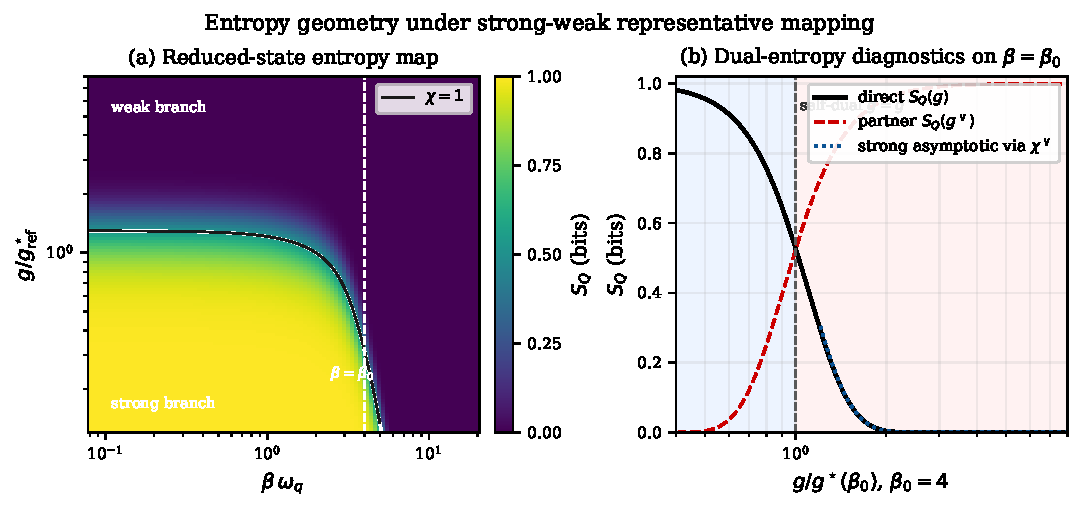
\includegraphics[width=\columnwidth]{../figures/hmf_spin_boson_entropy_duality.pdf}
  \caption{
  Entropy under strong-weak representative mapping.
  \textbf{(a)} Reduced-state entropy over \((\beta,g)\), with crossover contour \(\chi=1\).
  \textbf{(b)} At fixed \(\beta_0\), direct entropy \(S_Q(g)\), dual-partner entropy
  \(S_Q(g^\vee)\), and strong-branch asymptotic reconstruction in the dual coordinate \(\chi^\vee\).
  }
  \label{fig:spin_boson_entropy_duality_v2}
\end{figure}

\paragraph{Formal statements and proofs.}
The theorem-level forms of the strong-weak and orientation results used in this section are stated in
the Appendix.
